%%%%%%%%%%%%%%%%%%%%%%%%
%
%   Examples
%
%%%%%%%%%%%%%%%%%%%%%%%%

\chapter{Examples}

In the previous chapters a lot of different finite elements for different problems were introduced. The goal of this chapter will be to discuss some of the examples which can be found in the folders contained in \texttt{LehrFEM/Examples}. All of these folders contain files caled \texttt{main\_...}, which are routines that contain executeable code for different operators and problems.

In the discussion of the example problems some of the original code is inserted. A discussion of the code shown can always be found below the boxes.


\section{Linear and Quadratic finite elements} \label{sec:lqfe}

Probably the easiest example for a 2-dimensional finite element method is to use piecewise linear basis functions. This can be found in the folder \texttt{LehrFEM/Examples/QFE\_LFE}. The driver routine is called \texttt{main\_LFE}, the code can be found below.

\begin{lstlisting}
% Run script for piecewise linear finite element solver.

%   Copyright 2005-2005 Patrick Meury & Kah Ling Sia
%   SAM - Seminar for Applied Mathematics
%   ETH-Zentrum
%   CH-8092 Zurich, Switzerland
  
 % Initialize constants
   
 NREFS = 5;               % Number of red refinement steps
 F_HANDLE = @f_LShap;     % Right hand side source term
 GD_HANDLE = @g_D_LShap;  % Dirichlet boundary data
 GN_HANDLE = @g_N_LShap;  % Neumann boundary data
 
 % Initialize mesh
  
 Mesh = load_Mesh('Coord_LShap.dat','Elem_LShap.dat'); 
 Mesh.ElemFlag = ones(size(Mesh.Elements,1),1);         
 Mesh = add_Edges(Mesh);                                
 Loc = get_BdEdges(Mesh);
 Mesh.BdFlags = zeros(size(Mesh.Edges,1),1); 
 Mesh.BdFlags(Loc) = [-1 -2 -7 -7 -3 -4];
 for i = 1:NREFS
  Mesh = refine_REG(Mesh);     
 end
 Mesh = add_Edge2Elem(Mesh);
  
 % Assemble stiffness matrix and load vector
 
 A = assemMat_LFE(Mesh,@STIMA_Lapl_LFE);
 L = assemLoad_LFE(Mesh,P7O6(),F_HANDLE,0,1,2);
   
 % Incorporate Neumann boundary data
  
 L = assemNeu_LFE(Mesh,-1:-1:-4,L,gauleg(0,1,4),GN_HANDLE);
  
 % Incorporate Dirichlet boundary data
 
 [U,FreeDofs] = assemDir_LFE(Mesh,-7,GD_HANDLE);
 L = L - A*U;
  
 % Solve the linear system
 
 U(FreeDofs) = A(FreeDofs,FreeDofs)\L(FreeDofs);
    
 % Plot out solution
    
 plot_LFE(U,Mesh);colorbar;
 plotLine_LFE(U,Mesh,[0 0] ,[1 1]);
   
 clear all;
\end{lstlisting}

This routine solves the Laplace equation on an L-shaped domain with mixed boundary conditions (Neumann and Dirichlet) using linear finite elements.
\begin{align*}
 -\Delta u(x) &= f(x), \qquad && x\in \Omega \\
 u(x) &= g_D(x), && x \in \partial \Omega
\end{align*}
The stiffness matrix and the load vector are computed as discussed in Chapter \ref{chap:local_comp} and \ref{chap:assem}, the routines for linear finite elements are shown there as the reference example. The resulting linear system is solved in line 44. A plot of the solution on the computational domain is done in line 48. The solution along the line $(0,0),(1,1)$ is plotted in line 49.

The structure of the driver routine for using quadratic finite elements instead of linear finite elements looks very similar. Only the assembly routines and the function handles for computing local stiffness matrices have to be replaced. The name of the routine is \texttt{main\_QFE}.

The files \texttt{DiscrErrors\_...} in the same folder investigate the convergence rate of the used method. In these files the finite element solution is computed for problems, where the exact solution is known. This is done for several refinement steps, i.e. mesh widths. A part of the code for computing the convergence rate of linear and quadratic finite elements can be found below.

\begin{lstlisting}
%%%%%%%%%%%%%%%%%
% Initialize constants...
%%%%%%%%%%%%%%%%%

% Initialize mesh

Mesh = load_Mesh('Coord_Sqr.dat','Elem_Sqr.dat');
Mesh.ElemFlag = ones(size(Mesh.Elements,1),1);
Mesh = add_Edges(Mesh);
Loc = get_BdEdges(Mesh);
Mesh.BdFlags = zeros(size(Mesh.Edges,1),1);
Mesh.BdFlags(Loc) = -1;
for i = 1:NREFS
    
  % Do red mesh refinement  
    
  Mesh = refine_REG(Mesh);    
  Mesh = add_Edge2Elem(Mesh);
  
    
  % Assemble Stiffness matrix, load vector and incorporate BC

  A_QFE = assemMat_QFE(NewMesh,@STIMA_Lapl_QFE);
  L_QFE = assemLoad_QFE(NewMesh,P7O6(),F_HANDLE);
  
  A_LFE = assemMat_LFE(NewMesh,@STIMA_Lapl_LFE);
  L_LFE = assemLoad_LFE(NewMesh,P7O6(),F_HANDLE);
  
  % Incorporate Dirichlet and Neumann boundary data
       
  [U_LFE,FreeDofs_LFE] = assemDir_LFE(NewMesh,-1,GD_HANDLE);
  L_LFE = L_LFE - A_LFE*U_LFE;
  
  [U_QFE,FreeDofs_QFE] = assemDir_QFE(NewMesh,-1,GD_HANDLE);
  L_QFE = L_QFE - A_QFE*U_QFE;    
  
  % Solve the linear system

  U_LFE(FreeDofs_LFE) = A_LFE(FreeDofs_LFE,FreeDofs_LFE)\...
  			L_LFE(FreeDofs_LFE);
  U_QFE(FreeDofs_QFE) = A_QFE(FreeDofs_QFE,FreeDofs_QFE)\...
  			L_QFE(FreeDofs_QFE);
    
  % Compute discretization error
    
  LInf_Error_LFE(i) = LInfErr_LFE(NewMesh,U_LFE,U_EX_1);
  L2_Error_LFE(i) = L2Err_LFE(NewMesh,U_LFE,P7O6(),U_EX_1);
  H1S_Error_LFE(i) = H1SErr_LFE(NewMesh,U_LFE,P7O6(),U_EX_2);
  N_LFE(i) = size(NewMesh.Coordinates,1);
    
  LInf_Error_QFE(i) = LInfErr_QFE(NewMesh,U_QFE,U_EX_1);
  L2_Error_QFE(i) = L2Err_QFE(NewMesh,U_QFE,P7O6(),U_EX_1);
  H1S_Error_QFE(i) = H1SErr_QFE(NewMesh,U_QFE,P7O6(),U_EX_2);
  N_QFE(i) = size(NewMesh.Coordinates,1) + ...
  		size(NewMesh.Edges,1);
    
  h(i) = get_MeshWidth(Mesh);
    
end

%%%%%%%%%%%%%%%%%
% plot computed errors...
%%%%%%%%%%%%%%%%%
\end{lstlisting}

The variable \texttt{NREFS} specifies the number of refinement steps. In the loop starting in line 13 firstly the mesh is refined, then the matrices and the load vector assembled. With these it is possible to determine the finite element solution by solving a linear system. This is done for linear and quadratic finite elements. Since the exact solution is known the desired errors, i.e. $L^\infty$, $L^2$, $H^1$-seminorm can be computed (lines 44-55). After the loop one can plot the errors against the mesh width or the number of degrees of freedom using the data stored in the corresponding variables. Such a plot can be found in Figure \ref{fig:lfeqfe} for the solution of the Poisson equation on the square for the $L^2$ and the $H^1$-semi norm.

\begin{figure}[htb]
  \centering
  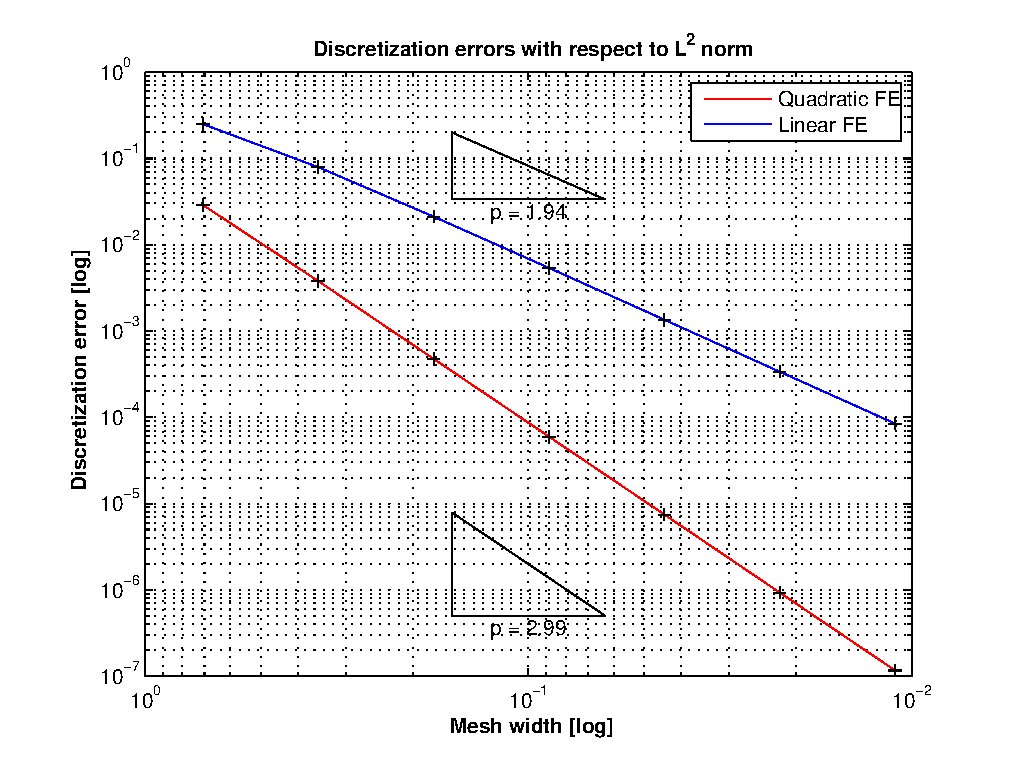
\includegraphics[width=0.7\textwidth]{L2lfeqfe.eps}
  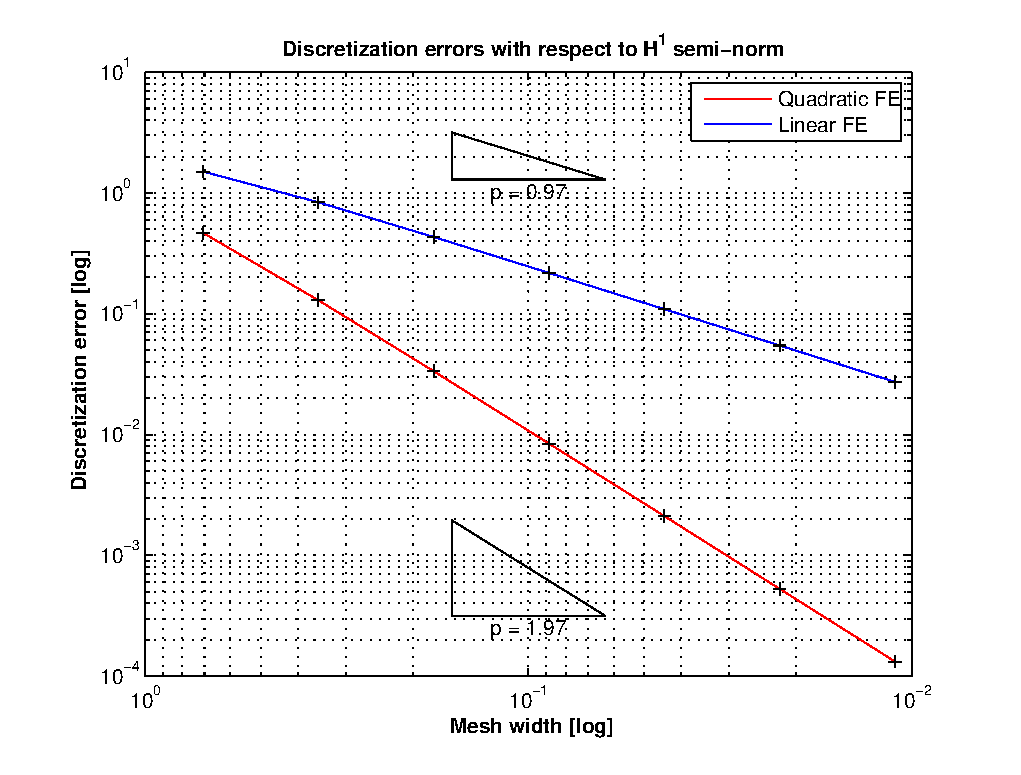
\includegraphics[width=0.7\textwidth]{H1lfeqfe.eps}
  \caption{Convergence rates for linear and quadratic finite elements}
  \label{fig:lfeqfe}
\end{figure}






\section{DG finite elements}

The driver routines for this method can be found in the folder \texttt{LehrFEM/Examples/DGFEM}. In the discontinuous galerkin method it is allowed to have discontinuities along the edges, therefore the underlying space of basis functions consists of the shape functions transformed to an arbitrary triangle using the uniquely defined linear affine transform. For example in the case of linear shape functions there are 3 degrees of freedom on every triangular element with vertices $(a_1,a_2,a_3)$, which are the uniquely determined linear functions satisfying $b_i(a_j)=\delta_{ij}$. This approach also affects the bilinear form, as described on p. \pageref{ssec:dg}.

The numbering of the degrees of freedom in this case is done elementwise, which means that the corresponding degrees of freedom to the element $i$ are given by $l(i-1)+(1,\ldots, l)$, where $l$ denotes the number of degrees of freedom on every element. The driver routine \texttt{main\_1} implements discontinuous Galerkin discretization using Crouzeix-Raviart elements. It solves the problem
\begin{align*}
 -\Delta u(x) &= f(x), \; x\in \Omega \\
 u(x) &= g_D(x), \; x\in \partial \Omega
\end{align*}
The code can be found below.

\begin{lstlisting}
% Run script for discontinuous Galerkin finite element solver.

%   Copyright 2006-2006 Patrick Meury
%   SAM - Seminar for Applied Mathematics
%   ETH-Zentrum
%   CH-8092 Zurich, Switzerland
  
% Initialize constants
  
% Number of red refinement steps
NREFS = 4;                                
% Right hand side load data
G = @(x,varargin)-4*ones(size(x,1),1);    
% Dirichlet boundary data
UD = @(x,varargin)x(:,1).^2+x(:,2).^2;    
% Symmetric (+1) or antisymmetric (-1) discretization
S = 1;                            
% Edge weight function 
SIGMA = @(P0,P1,varargin)10/norm(P1-P0);  
  
% Initialize mesh
  
Mesh.Coordinates = [-1 -1; 1 -1; 1 1; -1 1];
Mesh.Elements = [1 2 3; 1 3 4];
Mesh.ElemFlag = ones(size(Mesh.Elements,1),1);
Mesh = add_Edges(Mesh);         
Loc = get_BdEdges(Mesh);
Mesh.BdFlags = zeros(size(Mesh.Edges,1),1); 
Mesh.BdFlags(Loc) = -1;
for i = 1:NREFS
  Mesh = refine_REG(Mesh);
end
Mesh = add_Edge2Elem(Mesh);
Mesh = add_DGData(Mesh);
    
% Assemble matrices and load vectors
% (discontinuous Raviart elements)
   
QuadRule_1D = gauleg(0,1,2);
QuadRule_2D = P3O3();
  
[I1,J1,Avol] = assemMat_Vol_DG(Mesh,@STIMA_Lapl_Vol_DGCR);
  
[I2,J2,Jinn] = assemMat_Inn_DG(Mesh,@STIMA_InnPen_DGCR,SIGMA);
[I2,J2,Ainn] = assemMat_Inn_DG(Mesh,@STIMA_Inn_DGCR,S);
    
[I3,J3,Jbnd] = assemMat_Bnd_DG(Mesh,@STIMA_BndPen_DGCR,SIGMA);  
[I3,J3,Abnd] = assemMat_Bnd_DG(Mesh,@STIMA_Bnd_DGCR,S);
  
Lvol = assemLoad_Vol_DG(Mesh,@LOAD_Vol_DGCR,QuadRule_2D,G);
Lbnd = assemLoad_Bnd_DG(Mesh,@LOAD_Bnd_DGCR,...
		QuadRule_1D,S,SIGMA,UD);
    
% Create system matrix
       
A = sparse([J1; J2; J3; J2; J3], ...
           [I1; I2; I3; I2; I3], ...
           [Avol; Ainn; Abnd; Jinn; Jbnd]);
L = Lvol + Lbnd;
         
% Solve the linear system
  
U = A\L;
plot_DGCR(U,Mesh);
colorbar;
      
% Clear memory
  
clear all;
\end{lstlisting}

As described on pages \pageref{ssec:dg} and \pageref{ssec:ddg} the computation of the stiffness matrix is done in five steps (lines 42-49). The assembly of the load vector is done in the lines 50-52.

The driver routine \texttt{main\_2} determines the convergence rate for this method. The structure of the code is very similar to the convergence rate computation in the case of linear and quadratic finite elements which can be found in Section \ref{sec:lqfe}. Again one specifies the number of refinement steps and then the errors with respect to the exact solution are computed for different mesh widths.

Now we shall add a small description of the other driver routines contained in this folder.

\begin{itemize}
 \item \texttt{main\_0}: plots the mesh with the edge normals
 \item \texttt{main\_1}: explained above
 \item \texttt{main\_2}: explained above
 \item \texttt{main\_3}: solves the poisson equation on a square using linear finite elements
 \item \texttt{main\_4}: convergence rates on a square using linear finite elements
 \item \texttt{main\_5}: solves the poisson equation on a square using quadratic finite elements (number of degrees of freedom per element can be specified)
 \item \texttt{main\_6}: convergence rates on a square using quadratic finite elements (number of degrees of freedom per element can be specified)
 \item \texttt{main\_7}: as \texttt{main\_6} but with another exact solution
 \item \texttt{main\_8}: compares the convergence rates on a square for symmectric discretization and anti-symmetric discretization
\end{itemize}




\section{Whitney-1-forms}

The implemented examples using Whitney-1-forms can be found in the folder \texttt{Examples/W1F}. As already described in the chapters on local computations and assembly of the matrices the basis functions used are vector valued. Here the degrees of freedom are given by edge integrals. The driver routine called \texttt{main\_W1F} solves the problem
\begin{equation} \label{eq:ccurl}
 \nabla \times \mu_2 \, \nabla \times u + \mu_1 u = f
\end{equation}
for given functions $\mu_{1,2}$ and $f$. On the boundary solely Dirichlet conditions are enforced. The code can be found below.

\begin{lstlisting}
% Run script for W1F finite element solver.
%   Copyright 2005-2005 Patrick Meury & Mengyu Wang
%   SAM - Seminar for Applied Mathematics
%   ETH-Zentrum
%   CH-8092 Zurich, Switzerland

% Initialize constant
    
NREFS = 4;
MU1_HANDLE=@(x,varargin)1;
MU2_Handle = @(x,varargin)ones(size(x,1),1);
F_Handle = @(x,varargin)(pi^2+1)*[sin(pi*x(:,2)) ...
		sin(pi*x(:,1))];
GD_Handle = @(x,varargin)[sin(pi*x(:,2)) sin(pi*x(:,1))];

% Initialize mesh
    
Mesh.Coordinates = [-1 -1;1 -1;1 1;-1 1];
Mesh.Elements = [1 2 4;2 3 4];
Mesh = add_Edges(Mesh);
Mesh = add_Edge2Elem(Mesh);
Loc = get_BdEdges(Mesh);
Mesh.BdFlags = zeros(size(Mesh.Edges,1),1);
Mesh.BdFlags(Loc) = -1;
Mesh.ElemFlag = ones(size(Mesh.Elements,1),1);
    
for i=1:NREFS
   Mesh = refine_REG(Mesh);
end
    
% Assemble Curl-curl matrix, MASS matrix and load vector
t = cputime;
[IC,JC,C] = assemMat_W1F(Mesh,@STIMA_Curl_W1F,MU2_Handle,P7O6());
[IM,JM,M] = assemMat_W1F(Mesh,@MASS_W1F,MU1_HANDLE, P3O3());
A = sparse([IC;IM],[JC;JM],[C;M]);
L = assemLoad_W1F(Mesh,P7O6(),F_Handle);
    
% Incorporate Dirichlet boundary data
  
[U,FreeDofs] = assemDir_W1F(Mesh,-1,GD_Handle,gauleg(0,1,1));
L = L - A*U;
    
% Solve the system
    
U(FreeDofs) = A(FreeDofs,FreeDofs)\L(FreeDofs);
fprintf('Runtime of direct solver [s]  :  %f\n',cputime-t);

% Plot the solution

plot_W1F(U,Mesh);

clear all
\end{lstlisting}

The routine \texttt{main\_W1F2} solves the problem from \eqref{eq:ccurl} with an additional convective term, therefore the problem is given by
\begin{equation}
 \nabla \times \mu_2 \, \nabla \times u + v \times u + \mu_1 u = f.
\end{equation}
The function $v$ is some given velocity field.

The convergence rates for the above mentioned problems can be computed using the \texttt{Script\_W1F\_...} and \texttt{Script\_W1F2\_...} routines depending on the computational domain one is interested in.



\section{$hp$-FEM}

All the driver routines for the $hp$-FEM implementation can be found in the folder \texttt{Examples/hpFEM}. For further information on the theory behind the implementation see \cite{S04}. The basic structure is the same as in driver routines for other FEM. The code of the routine \texttt{main\_2}, which solves the Poisson equation on an L-shaped domain can be found below.

\begin{lstlisting}
% Runs script for hp-FEM.

% Copyright 2006-2006 Patrick Meury
% SAM - Seminar for Applied Mathematics
% ETH-Zentrum
% CH-8092 Zurich, Switzerland

% Initialize constants
  
NREFS = 10;                          
F = @(x,varargin)zeros(size(x,1),1); 
GD = @gD_LShap;                      
  
% Initialize mesh
 
Mesh = load_Mesh('Coord_LShap.dat','Elem_LShap.dat');
Mesh.ElemFlag = zeros(size(Mesh.Elements,1),1);
Mesh = add_Edges(Mesh);
Loc = get_BdEdges(Mesh);
Mesh.BdFlags = zeros(size(Mesh.Edges,1),1);
Mesh.BdFlags(Loc) = -1;  
  
CNodes = transpose(1:size(Mesh.Coordinates,1));
  
% Prepare mesh for longest edge bisection 
  
Mesh = init_LEB(Mesh);
for i = 1:NREFS
  Mesh = refine_hp(Mesh,CNodes);
end 
  
% Generate mesh data structure for hp-FEM

Mesh_hp.Coordinates = Mesh.Coordinates;
Mesh_hp.Elements = Mesh.Elements;
Mesh_hp.ElemFlag = zeros(size(Mesh_hp.Elements,1),1);
Mesh_hp = add_Edges(Mesh_hp);
Loc = get_BdEdges(Mesh_hp);
Mesh_hp.BdFlags = zeros(size(Mesh_hp.Edges,1),1);
Mesh_hp.BdFlags(Loc) = -1;
Mesh_hp = add_Edge2Elem(Mesh_hp);

% Assign polynomial degrees and build dof maps
  
[EDofs,CDofs,ElemDeg] = assign_pdeg(Mesh_hp,CNodes,NREFS);
Elem2Dof = build_DofMaps(Mesh_hp,EDofs,CDofs);
pmax = max(ElemDeg);

% Build shape functions and quadrature rules

QuadRule_1D = gauleg(0,1,2*pmax);
Shap_1D = shap_hp([QuadRule_1D.x zeros(size(QuadRule_1D.x))],pmax);
QuadRule_2D = Duffy(TProd(QuadRule_1D));
Shap_2D = shap_hp(QuadRule_2D.x,pmax);

% Assemble global load vector and mass matrix

A = assemMat_hp(Mesh_hp,Elem2Dof,...
	@STIMA_Lapl_hp,QuadRule_2D,Shap_2D);
L = assemLoad_hp(Mesh_hp,Elem2Dof,QuadRule_2D,Shap_2D,F);

% Incoporate Dirichlet boundary conditions
  
[U,FreeDofs] = assemDir_hp(Mesh_hp,Elem2Dof,...
			-1,QuadRule_1D,Shap_1D,GD);
L = L - A*U;
  
% Solve the linear system
  
U(FreeDofs) = A(FreeDofs,FreeDofs)\L(FreeDofs);
 
% Plot hp-FEM solution

plot_hp(U,Mesh_hp,Elem2Dof,pmax);
colorbar;
  
% Clear memory
  
clear all;
\end{lstlisting}

Here we shall give a description of the $hp$-FEM specific code segments.
\begin{itemize}
 \item In line 23 the corner nodes \texttt{CNodes} are specified. The refinement strategy implemented in the function \texttt{refine\_hp} (line 29) performs the largest edge bisection algorithm on all the elements sharing one of the nodes specified in \texttt{CNodes}.
 
 \item In the lines 43-47 the degrees of freedom are assigned to the elements and numbered. Firstly the function \texttt{assign\_pdeg} assigns the maximum polynomial degree to every element, which is then stored in the vector of length \texttt{nElements} called \texttt{ElemDeg}. Furthermore the vectors \texttt{CDofs} and \texttt{EDofs} are assigned, which have length \texttt{nElements} and \texttt{nEdges} respectively and contain the number of degrees of freedom on the edges and in the interior. The polynomial degree stored in \texttt{ElemDeg} increases linearly away from the corner nodes. Based on that the number of degrees of freedom on every edge and the internal degrees of freedom are computed. Then the function \texttt{build\_DofMaps} sets up the numbering of the degrees of freedom, which can then be found in the variable \texttt{Elem2Dof}. For details on the structure of this variable see below.
 
 \item In lines 49-54 the quadrature rules are set, for both 1D and 2D integrals. The accuracy of the quadrature rules is chosen in accordance to the maximal polynomial degree used in defining the finite element space. The shape functions in the quadrature points are pre-computed and then handled to all the functions using numerical integration. The shape functions are hierarchical (cf. Subsection \ref{ssect:shap_hp}), therefore they can be pre-computed even though different polynomial degrees are used.
 
 \item The assembly of the stiffness matrix and the load vector (lines 56-60) are done in the same spirit as for other finite elements. The assembly routine \texttt{assemMat\_hp} calls the function \texttt{STIMA\_Lapl\_hp} to compute the local element contributions and assembles the stiffness matrix making use of the numbering of the degrees of freedom stored in the variable \texttt{Elem2Dof}.
 
 \item A plot of the finite element solution can be done using the function \texttt{plot\_hp} (lines 74-75).
\end{itemize}

The variable \texttt{Elem2Dof} that is assigned in line 46 is a struct consisting of the following fields:
\begin{itemize}
 \item \texttt{EDofs}: is a cell array of length 3 containing information on the degrees of freedom on all 3 local edges; all of the cells are structs containing the fields
 \begin{itemize}
  \item \texttt{Dofs}: cell containing \texttt{nEldges} arrays, which contains the numbers of the degrees of freedom on the corresponding edge
  \item \texttt{nDofs}: vector of length \texttt{nEldges} with the number of degrees of freedom for every edge
  \item \texttt{Dir}: vector of length \texttt{nEldges} containing information about the direction of the local edges; $-1$ if the local edge has the same orientation as the global one and $1$ otherwise;
 \end{itemize}
 \item \texttt{CDofs}: is a struct containing the fields
 \begin{itemize}
  \item \texttt{Dofs}: cell containing \texttt{nElements} arrays, which contains the numbers of the inner degrees of freedom on the corresponding element
  \item \texttt{nDofs}: vector of length \texttt{nElements} with the number of inner degrees of freedom for every element
 \end{itemize}
 \item \texttt{tot\_EDofs}: contains the total number of degrees of freedom on all edges of the mesh
 \item \texttt{tot\_CDofs}: contains the total number of inner degrees of freedom on all elements of the mesh
\end{itemize}
To make this complicated structure more clear we shall give some examples. The input

\verb!>> Elem2Dof.EDofs{1}.Dofs{6}!

\noindent returns the numbers of degrees of freedom on the local edge with number $1$ on the element with number $6$. The inner degrees of freedom are called similarly. The call

\verb!>> Elem2Dof.CDofs.Dofs{6}!

\noindent returns the numbers of the inner degrees of freedom on the element number $6$. The numbers of degrees of freedom can be obtained by replacing \texttt{Dofs\{ 6\}} in the above lines by \texttt{nDofs(6)}.


Similarly to the routines for $hp$ finite elements one can also do just $p$ refinement, which means rising the polynomial degrees without refining the mesh. In this case the degrees of freedom are assembled differently. The code piece below replaces the lines 43-47 of the code above.

\begin{lstlisting}
EDofs = (pmax-1)*ones(size(Mesh.Edges,1),1);
if(pmax > 2)
  CDofs = (pmax-1)*(pmax-2)/2*ones(size(Mesh.Elements,1),1);
else
  CDofs = zeros(size(Mesh.Elements,1),1);
end

Elem2Dof = build_DofMaps(Mesh,EDofs,CDofs);  
\end{lstlisting}

The number of degrees of freedom on every element is chosen such that the corresponding shape functions form a basis of the space of polynomials of total degree $p_\text{max}$ on the element (cf. \cite{S04}). The variable \texttt{Elem2Dof} which contains all the information on the relation between the degrees of freedom and the elements is again a result of a call to the function \texttt{build\_DofMaps}.

There are also driver routines for visualizing the convergence rates of the $hp$-FEM. Since the theory tells us that for these finite elements we have
\begin{equation}
 \Vert u-u_N \Vert \leq C \; \exp(-b\sqrt[3]{N}),
\end{equation}
where $N$ denotes the degrees of freedom and $u_N$ denotes the corresponding finite element solution. Therefore we use linear scaling on the $x$-axis to draw $\sqrt[3]{N}$ and logarithmic scaling on the $y$-axis that shows the corresponding error. The line then has to be a line with slope $-b$. The result of the driver routine \texttt{main\_3}, which computes the discretization error on an L-shaped domain can be found in Figure \ref{fig:hp}.

\begin{figure}[htb]
  \centering
  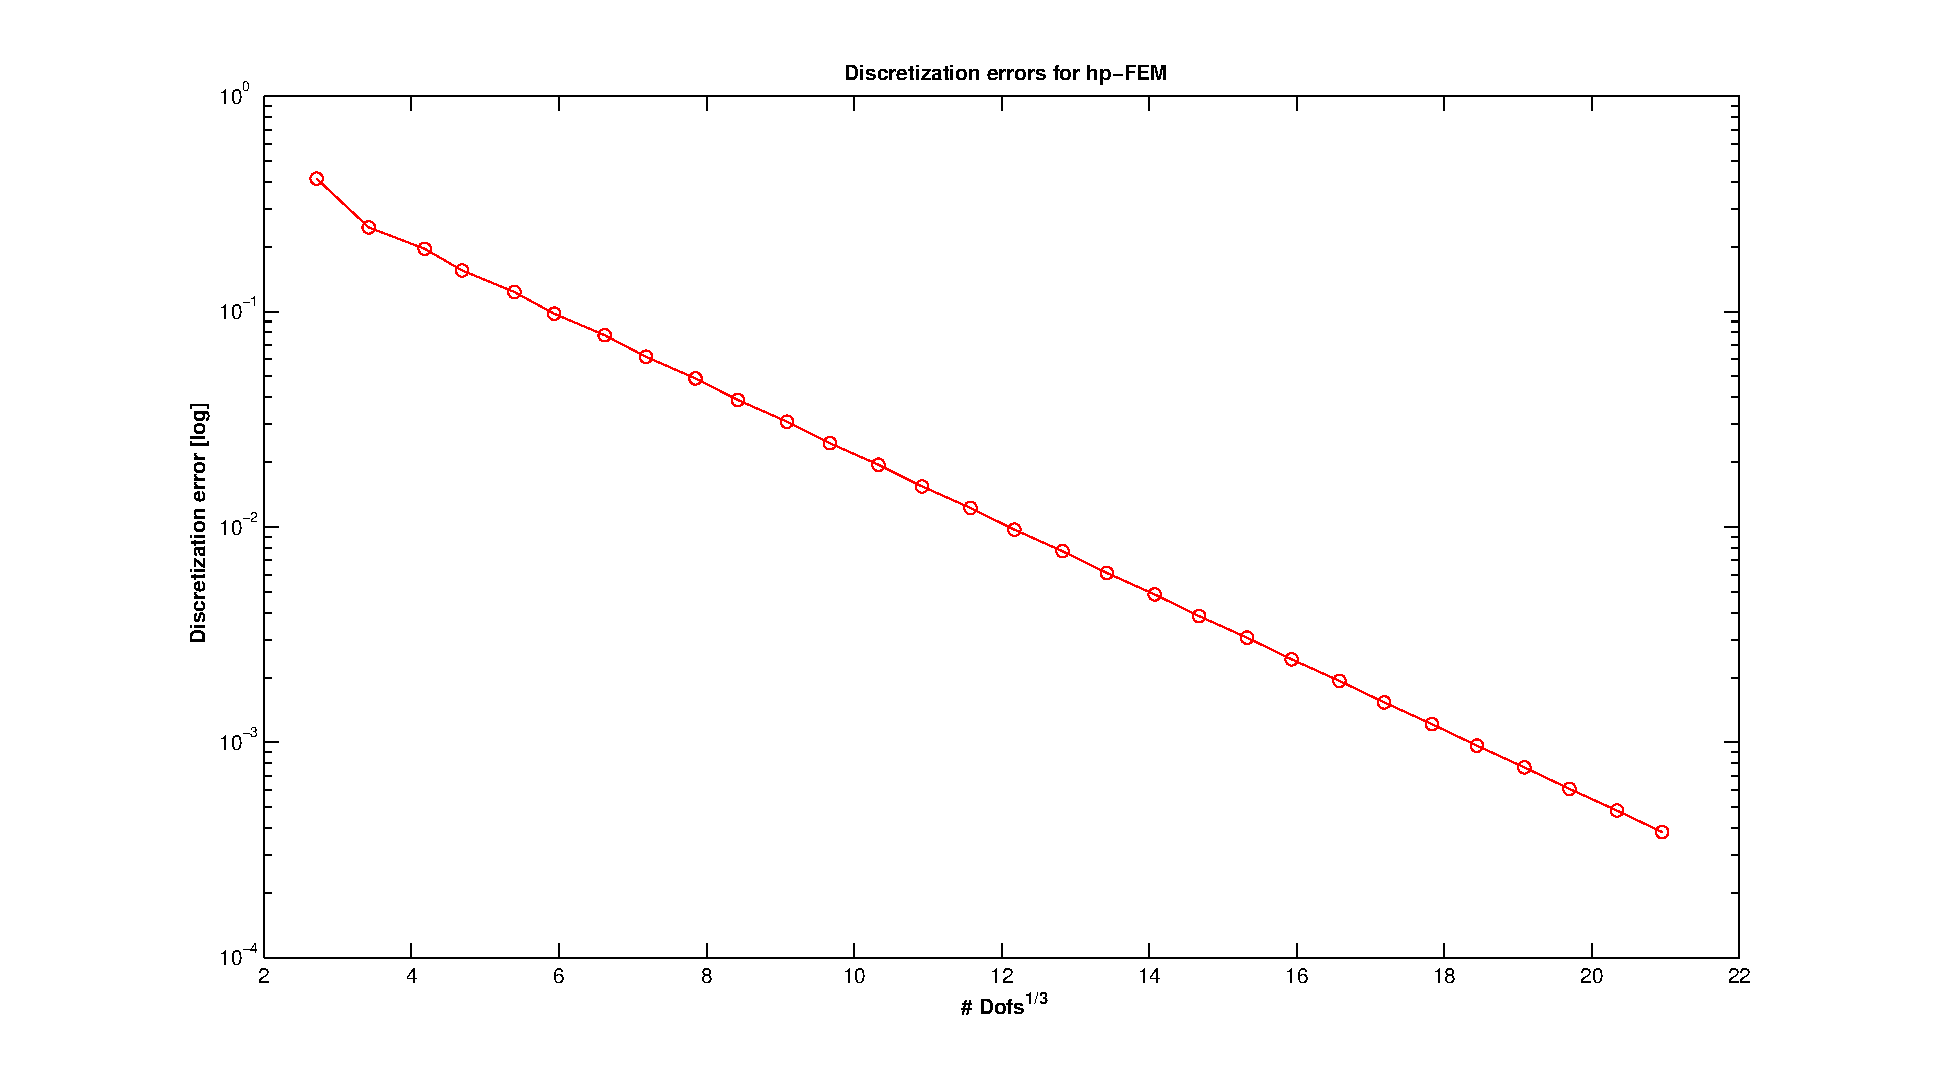
\includegraphics[width=0.9\textwidth]{hp.eps}
  \caption{Convergence rates for $hp$-FEM}
  \label{fig:hp}
\end{figure}



Now we shall give a short explanation of the other driver routines contained in this folder.

\begin{itemize}
 \item \texttt{main\_1}: Produces a plot that shows the distribution of the polynomial degrees on the mesh. The polynomial degree increases linearly away from the corner nodes (cf. \ref{ssec:asseMathp}).
 
 \item \texttt{main\_2}: explained in detail above
 
 \item \texttt{main\_3}: Computes the discretization error for different refinement steps to check convergence rates. The computational domain is L-shaped.
 
 \item \texttt{main\_4}: Convergence rates for $p-$refinement with an analytic solution on an L-shaped computational domain.
 
 \item \texttt{main\_5}: Solves the poisson equation on a square using $hp$-finite elements.
 
 \item \texttt{main\_6}: Convergence rate for $hp$-FEM on a square.
 
 \item \texttt{main\_7}: Convergence rate for $p$-refinement on a square.
 
 \item \texttt{main\_8}: Convergence rate for $p$-refinement on an L-shaped domain.
\end{itemize}






\section{Convection Diffusion problems}

The implementation of special methods for solving convection diffusion equations with a dominating convective term can be found in the folder \texttt{Examples/DiffConv}. In addition to the finite element based methods there is also an implementation of the finite volume method availlable (cf. Chapter \ref{chapt:fvm_conv_diff}).

The convection diffusion equations we look at have no time dependecy and are of the form
\begin{equation}
 -a \Delta u + c \cdot \nabla u = f,
\end{equation}
where $f:\Omega\to\mathbb{R}$ and $c:\Omega\to\mathbb{R}^2$. We assume $a$ to be a real number. The problems we want to investigate have a dominating convective term, i.e. $a$ should be small compared to the magnitude of the velocity field $c$. In the implementation the diffusion constant is of order $10^{-10}$, while both components of $c$ are of order $10^0$. Different methods are implemented for the discretization of the convection term $c\cdot \nabla u$ in the equation. It is well known that for this kind of problem a standard finite element discretization yields very bad results even though the results on convergence rates apply. This is due to large constants in the estimates. The weak form is given by
\begin{equation}
 \int_\Omega (a \nabla u \cdot \nabla v + (c\cdot \nabla u)v) \; dx = \int_\Omega fv \; dx.
\end{equation}
Apart from the standard finite element approach we want to discuss two other methods to overcome the difficulties.

\subsection{SUPG-method}
The second approach is the so called \textit{streamline upwind Petrov-Galerkin method (SUPG-method)}. For details see \cite{KA00},\cite{S08}. The basic idea is to use the identy
\begin{equation} \label{eq:supgg}
 \sum_{K} \delta_K \langle -a \Delta u + c \cdot \nabla u,\tau(v)\rangle = \sum_K \delta_K \langle f,\tau(v)\rangle_K,
\end{equation}
where $\langle \cdot,\cdot \rangle_K$ denotes the $L^2$ inner product on the elment $K$. The identity above holds in the $L^2$ sense and requires further assumptions on the smoothness of the solution $u$. Furthermore the identity is true for any choice of parameters $\delta_K$. The summation runs over all elements of the mesh. The mapping $\tau:L^2 \rightarrow L^2$ assigns a function to every test function $v$. This identity is added to the standard finite element discretization for stabilization purposes. The SUPG-method correlates to the choice $\tau(v)=c \cdot \nabla v$. For the special case of linear finite elements the bilinear form can then be written as
\begin{equation}
 a(u,v)=\int_\Omega (a \nabla u \cdot \nabla v) \; dx + \langle c \cdot \nabla u,v\rangle + \sum_K \delta_K \langle c \cdot \nabla u, c \cdot \nabla v\rangle_K.
 \label{eq:supg}
\end{equation}
where $\langle \cdot,\cdot \rangle$ denotes the $L^2$ inner product on the computational domain $\Omega$. The corresponding left hand side is given by the linear functional
\begin{equation}
 l(v)= \left\langle f,v \right\rangle + \sum_K \delta_K \langle f,c \cdot \nabla v\rangle_K
\end{equation}



\subsection{Upwinding methods}
Finally the third approach is done by so called upwinding schemes to discretize the convection term. The diffusion term is discretized in the standard finite element manner. Here we shall only give a short outline of the idea, more information can be found in \cite{S08}. To evaluate the stiffness matrix corresponding to the convective term $\langle c \cdot \nabla u,v\rangle$ we have to approximate integrals of the form
\begin{equation} \label{eq:upw1}
 \int_T (c \cdot \nabla \varphi_j)\varphi_i \; dx,
\end{equation}
where $\varphi_i$ are basis functions in the used finite element space. In the standard finite element approach this is done by Gaussian integration. Here we also use an integration rule on an element, which in general can be formulated as
\begin{equation}
 \int_T f(x) \; dx \approx |T|\sum_i w_i f(x_i),
\end{equation}
for given weights and evaluation points. In the case of the convective term the integrand from \eqref{eq:upw1} can be inserted in the integration formula. Doing this the term $(c \cdot \nabla \varphi_j)(x_i)$ appears. For points in the interior of the element this value is simply computed using the shape functions. For points on the boundary $\nabla \varphi_j$ might have a jump. An upwinding triangle for the boundary point $x$ is then defined as a triangle $T$ where the vector $-c(x)$ points into. Possibly there are more upwinding triangles but in this case one can just use any of them. Then take $\nabla \varphi_j(x)$ to be the limiting value coming from the corresponding upwinding triangle.

This kind of upwinding method is implemented for linear and quadratic finite elements. We will have a closer look at the easier linear finite elements. The quadratic case is treated similarly, but involves more quadrature points. In the reference routine we want to look at the quadrature points are placed on the mid points of the edges and the corresponding weights are all $1/3$. When computing the stiffness matrix on an element the convection contribution for two basis functions has to be evaluated as shown in \ref{eq:upw1}. By the definition of the upwind quadrature the term $(c \cdot \nabla \varphi_j)(m)$ evaluates to the same value for both triangles $T_1$ and $T_2$ sharing the edge with the midpoint $m$. This can be expoited when computing the local stiffness matrices by computing the value $(|T_1|+|T_2|)/3 \; (c \cdot \nabla \varphi_j)(m)\varphi_i(m)$. The code for computing the stiffness on an element can be found below.

\begin{lstlisting}
function UP_loc = STIMA_UPLFE(Vertices,vHandle, mass, varargin)
%   Copyright 2007 Holger Heumann
%   SAM - Seminar for Applied Mathematics
%   ETH-Zentrum
%   CH-8092 Zurich, Switzerland

UP_loc = zeros(3,3);
 
x=[0.5 0; 0.5 0.5; 0 0.5];
 
% Compute element mapping

a1 = Vertices(1,:);
a2 = Vertices(2,:);
a3 = Vertices(3,:);
  
m1=(a2+a1)/2;
m2=(a3+a2)/2;
m3=(a1+a3)/2;
    
bK = a1;
BK = [a2-bK; ...
      a3-bK];
det_BK = abs(det(BK));
inv_BK = inv(BK); 
  
% Compute gradient of local shape functions
  
gradN=grad_shap_LFE(x);
for i=1:2:6
    gradN(:,[i i+1])=gradN(:,[i i+1])*inv_BK';
end
  
% Extract nodal vectors
    
v = -vHandle(x*BK + ones(3,1)*a1);
  
%Compute Lie derivative scheme for first
% midpoint using upwind quadrature    
yhat = (m1+v(1,:)-bK)*inv_BK;
if(yhat(2) >= 0)
  elem= mass(1)/2*[-gradN(1,[1 2])*v(1,:)',...
             -gradN(1,[3 4])*v(1,:)',...
             -gradN(1,[5 6])*v(1,:)'];
  UP_loc(1,:) = elem; 
  UP_loc(2,:) = elem;
end
if (yhat(2)==0)
   UP_loc(1,:)=1/2* UP_loc(1,:);
   UP_loc(2,:)=1/2* UP_loc(1,:); 
end
  
% Compute Lie derivative scheme for second
% midpoint using upwind quadrature
yhat = (m2+v(2,:)-bK)*inv_BK;
if(sum(yhat) <= 1)
  elem = mass(2)/2*[-gradN(2,[1 2])*v(2,:)', ...
              -gradN(2,[3 4])*v(2,:)', ...
              -gradN(2,[5 6])*v(2,:)'];
  UP_loc(3,:) = UP_loc(3,:)+elem;
  UP_loc(2,:) = UP_loc(2,:)+elem;
end
if (sum(yhat)==1)
   UP_loc(2,:)=1/2* UP_loc(2,:);
   UP_loc(3,:)=1/2* UP_loc(3,:);
end
  
% Compute Lie derivative scheme for third midpoint
% using upwind quadrature
yhat = (m3+v(3,:)-bK)*inv_BK;
if(yhat(1) >= 0)
  elem = mass(3)/2*[-gradN(3,[1 2])*v(3,:)', ... 
              -gradN(3,[3 4])*v(3,:)', ...
              -gradN(3,[5 6])*v(3,:)'];
  UP_loc(3,:) = UP_loc(3,:)+elem;
  UP_loc(1,:) = UP_loc(1,:)+elem;
end
if (yhat(1)==0)
   UP_loc(1,:)=1/2* UP_loc(1,:);
   UP_loc(3,:)=1/2* UP_loc(3,:);
end

return
\end{lstlisting}

The input parameter \texttt{mass} is a vector of length $3$. The $i$-th entry contains one third of the area of the two elements sharing the local edge $i$. In the lines 38-51 the local computations are done for the first midpoint $m_1$, which lies in between the vertices $a_1$ and $a_2$. If the current triangle is an upwinding triangle with respect to $m_1$ we can compute the value
\begin{equation}
 \frac{|T_1|+|T_2|}{3} (c \cdot \nabla \varphi_j)(m_1)\varphi_i(m_1).
\end{equation}
The basis functions corresponding to the nodes $a_1$ and $a_2$ evaluate to $1/2$ while the one corresponding to $a_3$ is zero in $m_1$. This leads to the computations in lines 42-46. If both triangles are upwinding triangles the contribution has to be multiplied by $1/2$, which is done in the lines 49 and 50. The same computations are perfomed for the other midpoints.

The assembly of the global stiffness matrix for the upwinding discretization of the convective term is done in the routine \texttt{assemMat\_UpLFE}.


\subsection{The driver routines}

As reference driver routine we chose \texttt{main\_error0Flfe}, the code of which can be found below.

\begin{lstlisting}
% Initialize constants
  

JIG=2;
d1=1;             %impact of supg modification
d2=1;
a=10^-10          %amount of diffusivity
NREFS =7;

% select test code
d=getData(5);
     
QuadRule = P7O6(); 
  
Mesh.Coordinates =d.Coordinates; 
Mesh.Elements = d.Elements;
Mesh = add_Edges(Mesh);
Loc = get_BdEdges(Mesh);
Mesh.BdFlags = zeros(size(Mesh.Edges,1),1);
sh.BdFlags(Loc) = d.boundtype;
Mesh.ElemFlag = ones(size(Mesh.Elements,1),1);
  
err=zeros(NREFS,5);
err1=zeros(NREFS,5);
h=zeros(NREFS,1);
Dofs=zeros(NREFS,1);
  
for i = 1:NREFS
 %refine Mesh   
 Mesh = refine_REG(Mesh);
 Mesh=add_Edge2Elem(Mesh);
        
  
 %Laplace
 A = assemMat_LFE(Mesh,@STIMA_Lapl_LFE,P3O3());
   
 UP4=assemMat_UpLFE(Mesh,d.V_Handle);
 B_supg=assemMat_LFE(Mesh,@STIMA_SUPG_LFE,P3O3(),...
 		 d.V_Handle,a,d1,d2);
 B=assemMat_LFE(Mesh,@STIMA_Conv_LFE,d.V_Handle,P7O4());

 A_u4=a*A+(UP4);
 A_supg=a*A+B+B_supg;
 A_s=a*A+B;
 
 L = assemLoad_LFE(Mesh,P3O3(),d.SOL_Handle,a);
 L_supg=assemLoad_LFE_SUPG(Mesh,P3O3(),...
 		d.V_Handle,d.SOL_Handle,a,d1,d2);
   
 %Incorporate Dirichlet boundary data
   
 [U_s,FreeDofs] = assemDir_LFE(Mesh,[-1 -2],d.U_EX_Handle,a);
 U_u4=U_s;
 U_supg=U_s;
    
 L_u4 = L - A_u4*U_u4;
 L_s = L - A_s*U_s;
 L_supg = L+L_supg - A_supg*U_supg;
   
 % Solve the linear system
 
 U_u4(FreeDofs) = A_u4(FreeDofs,FreeDofs)\L_u4(FreeDofs);
 U_s(FreeDofs) = A_s(FreeDofs,FreeDofs)\L_s(FreeDofs);
 U_supg(FreeDofs)=A_supg(FreeDofs,FreeDofs)\L_supg(FreeDofs);
   
 err1(i,4)=L2Err_LFE(Mesh,U_u4,P7O6(),d.U_EX_Handle,0,a);
 err1(i,5)=L2Err_LFE(Mesh,U_s,P7O6(),d.U_EX_Handle,0,a);
 err1(i,6)=L2Err_LFE(Mesh,U_supg,P7O6(),d.U_EX_Handle,0,a);

 Dofs(i)=size(Mesh.Coordinates,1); 
 plot_LFE(U_u4,Mesh); colorbar
end 
 
%%%%%%%%%%%%%%%%%
% plot computed errors...
%%%%%%%%%%%%%%%%%
  
clear all;
\end{lstlisting}

The driver routine above compares the convergence rates of 3 different methods. The stiffness matrix for the standard finite element discretization is computed as the sum of the discretized convective and diffusive term in line 44. The right hand side for this method is assembled in line 46.



The matrix that is added to the original stiffness matrix based on the additional term apearing in \eqref{eq:supg} correlated with the SUPG method is computed in line 38. The final system matrix is then computed in line 43. The right hand side also consists of two contributions now, the original right hand side and the right hand side of \eqref{eq:supgg}. The computation is done in the lines 47 and 58. The solution is then computed in line 64.


The stiffness matrix resulting from an upwind discretization is computed in line 37, the corresponding finite element solution is computed in line 62.

The plot of the errors is omited in this code sample since it does not involve any code that is related to the presented methods. The output of the \texttt{main\_error0Flfe} can be found in Figure \ref{fig:convdiff}. Other driver routines in this folder shall be explained in the following.

\begin{figure}[htb]
  \centering
  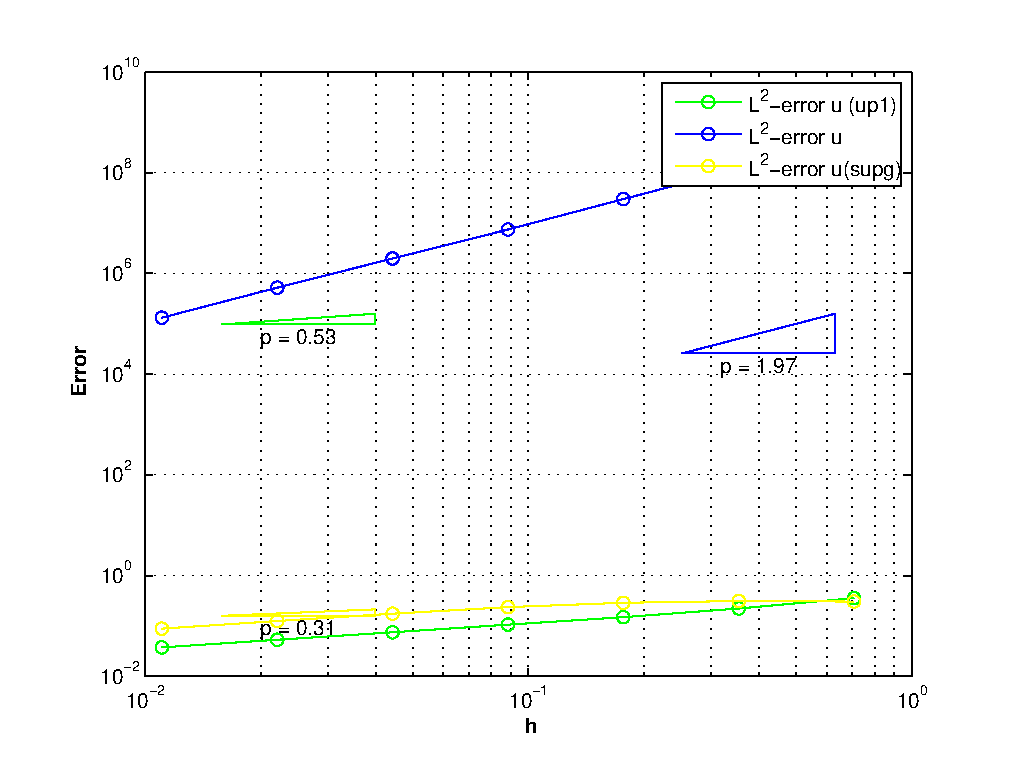
\includegraphics[width=0.9\textwidth]{main_error0Flfe.eps}
  \caption{Convergence rates for a convection diffusion problem}
  \label{fig:convdiff}
\end{figure}

\begin{itemize}
 \item \texttt{LFE\_invNorms} compares different discretization methods for different amount of diffusivity.
 \item \texttt{main\_error} compares different discretization methods for different mesh widths. For upwinding the vertices are used as quadrature points.
 \item \texttt{main\_error0Fqfe} compares different discretization methods for different mesh widths. Quadratic finite elments are used and the quadrature points are the vertices, the midpoints and one center point.
 \item \texttt{QFE\_invNorms} compares different discretization methods for different amount of diffusivity using quadratic finite elements.
\end{itemize}











